
% this file is called up by thesis.tex
% content in this file will be fed into the main document

%: ----------------------- introduction file header -----------------------
% the code below specifies where the figures are stored
\graphicspath{{6/figures/}}

\chapter{From Music Audio to Guitar Tablature}
\label{chp:background}

Automatic chord recognition is conventionally tackled as a general music audition task, where the desired output is a time-aligned sequence of discrete chord symbols, e.g. CMaj7, Esus2, etc.
In practice, however, this presents two related challenges:  one, the act of decoding a given chord sequence requires that the musician knows both the notes in the chord and how to play them on some instrument; and two, chord labeling systems do not degrade gracefully for users without significant musical training.
Alternatively, we address both challenges by modeling the physical constraints of a guitar to produce \emph{human-readable representations} of music audio, i.e guitar tablature via a deep convolutional network.
Through training and evaluation as a standard chord recognition system, the model is able to yield representations that require minimal prior knowledge to interpret, while maintaining respectable performance compared to the state of the art.


\section{Background}
\label{sec:part1}

Given sustained effort and interest by the research community, automatic chord recognition is now one of the seminal tasks in music informatics.
As the state of the art has advanced, most approaches adopt the same basic architecture: first, acoustic features, known as pitch class profiles or chroma, are computed from short-time observations of an audio signal \cite{Fujishima1999}; then, Gaussian mixture models (GMMs) are fit to each chord class in the target vocabulary, typically 12 Major, 12 Minor, and one waste-basket ``no-chord'' class \cite{Bello2005}; finally, frame-wise predictions are decoded using a Hidden Markov Model with transition probabilities computed from the same data used for training the GMMs \cite{Sheh2003}.
Alternatively, deep learning methods have recently garnered attention for chord recognition, such as convolutional neural networks (CNNs)\cite{Humphrey2012} and recurrent neural networks (RNNs) \cite{Boulanger2013}.

\begin{figure}[t!]

  \centering
  \centerline{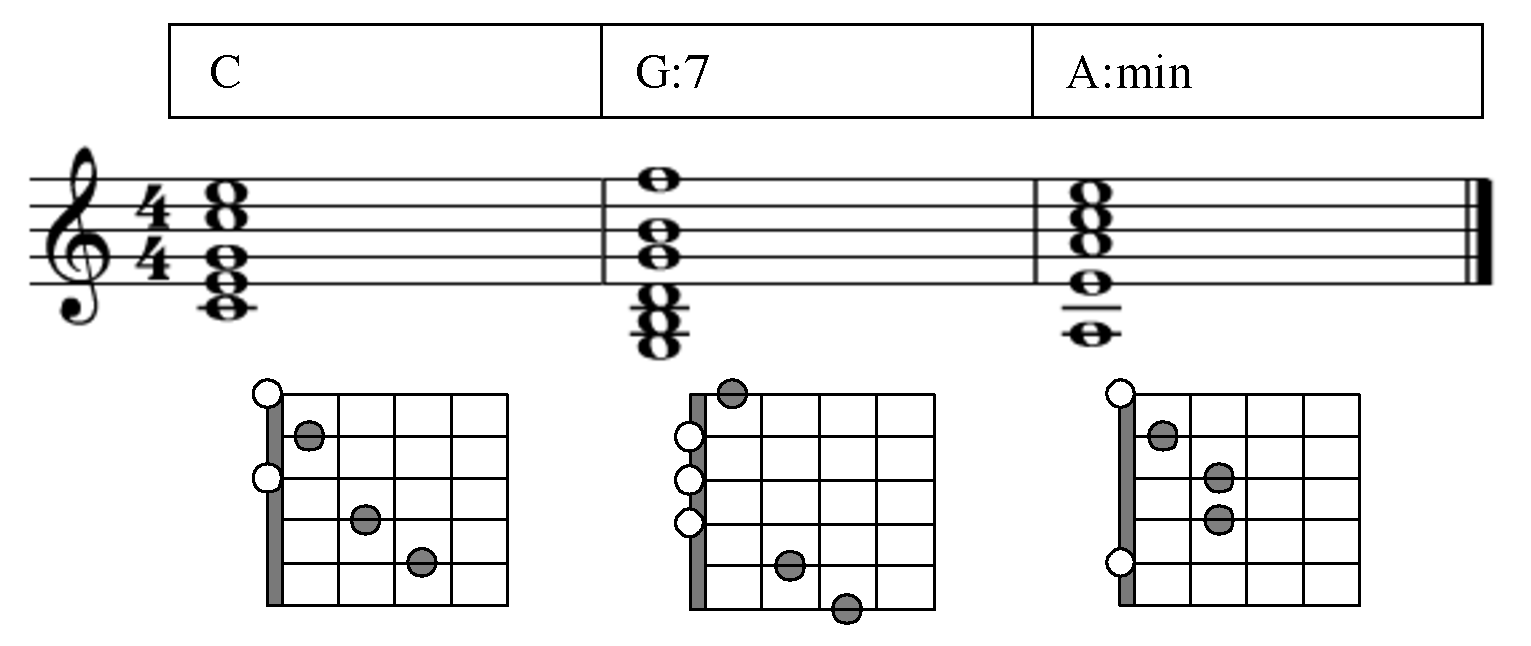
\includegraphics[width=3.25in]{chord_tablature}}
\caption{A chord label sequence (top), traditional staff notation (middle), and guitar tablature (bottom) of the same musical information, in decreasing levels of abstraction.}
\label{fig:different_notation}
%
\end{figure}


Generally speaking, the majority of prior research in automatic chord recognition is based on the two-fold premise that (a) this is fundamentally a classification problem and (b) the ideal output is a time-aligned sequence of singular chord names, motivated by the spirit of empowering anyone to play any song.
Modern online guitar communities, however, have continued to place a high demand on guitar tablature, given the prevalence of user-curated websites like Ultimate Guitar\footnote{http://www.ultimate-guitar.com/}, which sees an average 1.7M unique visitors in the US per month\footnote{Based on Compete.com analytics data, accessed on 2 November, 2013.}.
As illustrated in Figure \ref{fig:different_notation}, guitar tablature is a form of music notation that requires minimal knowledge to interpret because the representation directly maps notes in a chord to frets on a guitar.
Therefore, it is an inherent design challenge of human-facing expert systems that the output must be easily interpreted by the user; and, more importantly, graceful degradation is a function of that user's capacity to understand and recover from errors.
Though some previous work embraces this position in the realm of transcribing guitar recordings \cite{Barbancho2012} or arranging music for guitar \cite{Hori2013}, there is, to our knowledge, no existing work in estimating guitar tablature directly from polyphonic recordings.

%emits chord names is that the end user must have the prerequisite knowledge to make musical sense of this information;

% This paper presents a novel approach to bootstrapping the task of automatic chord recognition to develop an end-to-end system capable of representing polyphonic music audio as guitar tablature by modeling the mechanics of the guitar with a deep convolutional network.
% To enforce playability, a finite vocabulary of chord shape templates are defined and the network is trained by minimizing the distance between its output and the best template for an observation.
% Our experiments show that the model achieves the goal of faithfully mapping audio to a fretboard representation, while still performing respectably as a chord recognition system.
% The output of the network is human-readable, allowing the system to be used by anyone regardless of musical ability.
% Additionally, trained networks are not constrained to any particular vocabulary, and are able to represent previously unseen chord shapes.

\section{System Design Considerations}

Much of this work proceeds directly from previous efforts in automatic chord estimation.
The input leverages the same CQT representation, and is omitted from the discussion here.


\subsection{Designing a Fretboard Model}
\label{subsec:design}

Deep trainable networks have proven to be a versatile, powerful, and practical approach to solving complex machine learning problems in a variety of fields.

\begin{figure}[t!]
  \centering
  \centerline{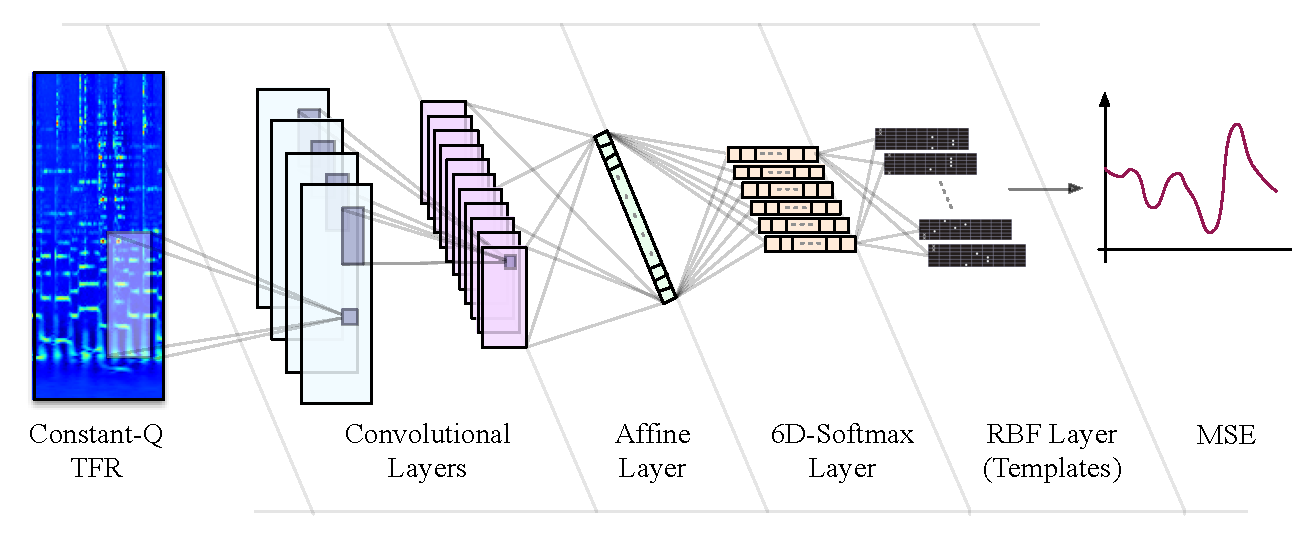
\includegraphics[width=3.5in]{sys_diagram}}
%  \vspace{1.5cm}
\caption{Full diagram of the proposed network during training.}
\label{fig:sys_diagram}
%
\end{figure}


Finally, the last layer, $f_3$, that produces the fretboard-like output, $Z_{out}$, is defined similarly to $f_2$, with the exception that $W$ is now a tensor, and the result of each matrix-vector product is normalized by the softmax operation, defined as:

\begin{equation}
\label{eq:softmax}
\small
\sigma(x)=\frac{\exp(x)}{ \sum_{m=1}^M\exp{(x[m])}}
\end{equation}

\noindent This layer is then given by the following:

\begin{equation}
\label{eq:softmax_layer}
\small
f_3(X_{3} \vert \theta_3) = \sigma (h( W[k] \bullet X_{3} + b)), k \in [0:K), \theta_3 = [W, b]
\end{equation}

\noindent Again, as in the previous layer, the input is a flat vector of length $N$, but the weights are now a tensor of shape $(K,M,N)$ and the bias is a matrix with shape $(K,M)$.
This layer is equivalent to performing $K$ parallel affine transformations, each normalized by the softmax function.
The intuition for this design is straightforward; a guitar consists of a finite number of strings, and, because the instrument is fretted, each can only be pressed at one of a few discrete positions on the neck.
In this way, the $K$-parallel softmax surfaces behave like probability mass functions for each string of the guitar, and the output $Z_{out}$ is shaped $(K, M)$.



\subsection{Chord Shape Vocabulary}
\label{subsec:vocabulary}

In this work,we consider five chord qualities (maj, min, maj7, min7 and 7) in all 12 pitch classes, plus one no-chord class, for a total of 61 classes.
Chord shapes are designed such that all qualities with the same root are formed in same neck position, as seen in the first column of Figure \ref{fig:fretboard_predictions}.
Consequently, all chords with the same root will be near-neighbors in this representation, and we should expect that the most common confusions will occur between qualities.
Additionally, though guitar chords can be voiced in variety of ways, here we consider a single shape for each as an initial simplification.
%It is worth mentioning that the guitar, as opposed to say, a piano, can play approximately the same chord in a variety of positions.
%However, mapping these multiple voicings for the same chord would require an additional layer, and for now we only consider a single template for each chord as a simplification.

\subsection{Loss Function}
\label{subsec:loss}

Having designed a fretboard model, we turn our attention to designing a loss function such that the machine can learn to faithfully reproduce it.
Following the lead of \cite{LeCun1998}, we train the network through an additional Radial Basis Function (RBF) layer, given as follows:

\begin{equation}
\small
\mathcal{L}(Z_{out} \vert W_T) = \sum(Z_{out} - W_{T}[i])^2
\end{equation}

\noindent where $Z_{out}$ is the output of the fretboard model, $W$ is a tensor of chord shape templates with shape $(C,K,M)$, $C$ is the number of chord shapes, and $i$ is the index of the correct class.
Note that these templates will impose the proper organization on the output of the model, and thus remain fixed during the learning process.
Since these weights are constant, minimizing this function does not require a contrastive penalty or margin term to prevent it from collapsing, i.e. making all the squared distances zero.


\subsection{Training Strategy}
\label{subsec:strategy}

For training the model, we use mini-batch stochastic gradient descent with a constant learning rate of 0.02.
When sampling the data, each observation is circularly shifted in pitch randomly on the interval [-12,12].
This allows the variance of each chord quality to be evenly distributed across classes, effectively turning the task into a 6-class problem as each datapoint contributes equally to pitch class.
Empirically, we observed that a mini-batch with a uniform quality distribution led to poor discrimination of Major chords.
This is likely due to the wide intra-class variance of major chords, which we offset by constituting batches with 3 Major observations for 1 of each other quality, and use a total batch size of 64 (24 Major, 8 Minor, 8 no-chord, etc).


\section{Methodology}

In lieu of measuring subjective experience of using the system, we evaluate the quality of this model in the context of chord recognition.
To also quantify the impact of the guitar-specific constraints, we define a second model with the same parameter complexity outlined in Subsection \ref{subsec:params}, but modify the transformation of $f_3$ to be a fully-connected layer like $f_2$ and use a linear softmax classifier rather than the RBF-templates, trained to minimize the negative log-likelihood.
This allows us to control for model complexity and determine the influence of the design constraints on the learning problem.
Both models are run for 30k iterations.
